\section{Evaluation}

In this section we provide experiments\footnote{Sources of benchmarking automation infrastructure: \url{https://github.com/vkutuev/matrix-benchmark}.} with Brahma.FSharp platform which are aimed to demonstrate its main features on regular (not HPC) devices\footnote{Looks more suitable for business applications that use .NET.}. 
We evaluated Brahma.FSharp in two cases listed below and described in respective sections.
\begin{enumerate}
\item The first one is an image convolution that demonstrates utilization of several GPU-s using F\# MailboxProcessor.
\item Second one is a matrix multiplication that demonstrates ability to create generic strongly statically typed kernels, to utilize local and private memory for performance optimization, and to demonstrate portability across different devices.
\end{enumerate}


\subsection{Image Convolution}

We implement image convolution in order to demonstrate multiple GPGPUs utilization.
Native for F\# asynchronous model, as was shown in~\cite{aleaGPUasync}, simplifies creation of complex workflows that include computations on GPGs.
We use F\# MailboxProcessor because Brahma.FSharp provides it as an interface for communication with GPUs.
Kernel is simply wrapped as shown in~\ref{lst:img_conv}. 
Simple load balancer that send next image to an agent with less number of messages in the input queue was implemented.

\begin{listing}[h]
  \begin{minted}[linenos]{fsharp}
let imgProcessor filter (imgSaver: MailboxProcessor<_>) =
    MailboxProcessor.Start(fun inbox ->
        let rec loop ... = async { // Async message processing loop
            let! msg = inbox.Receive() // Load message
            match msg with
            | EOS ch -> // Handle end of stream
                imgSaver.PostAndReply EOS
                ch.Reply()
            | Img img -> // Handle image
                let filtered = filter img // Convolution
                imgSaver.Post (Img filtered)
                return! loop ... }// Got to next message
        loop ...)
  \end{minted}
  \caption{MailboxProcessor-based wrapper for kernel to make it easier to integrate it to complex workflow}
  \label{lst:img_conv}
\end{listing}

We evaluate this solution on a \textbf{Lenovo} platform with two GPUs: NVIDIA GeForce MX150 and Intel(R) UHD Graphics 620.
We assume that all images are loaded into RAM and converted to grayscale. 
Typical chain of filters is applied: 3 Gaussian blur ($5 \times 5$ kernel), then edges detection ($5 \times 5$ kernel).
420 images (1gb of data) was handled in 40 seconds with two GPUs, in 64 seconds using Nvidia GPU only, and in 97 seconds using Intel GPU only.
Thus we can see that even naive multi-GPU workflow allows one to achieve up to 30\% speedup.

\subsection{Matrix Multiplication}

We evaluate generic kernel parametrized by types and operations (see listing~\ref{lst:mXm_kernels}), implemented in F\#.
Several basic optimizations, inspired by ``Tutorial: OpenCL SGEMM tuning for Kepler'' by Cedric Nugteren\footnote{``Tutorial: OpenCL SGEMM tuning for Kepler'': \url{https://cnugteren.github.io/tutorial/pages/page1.html}}, were applied.
Namely, we use tiling in local and private memory.
But current version supports only square matrices and square tiles.

\begin{figure}
  \begin{center}
  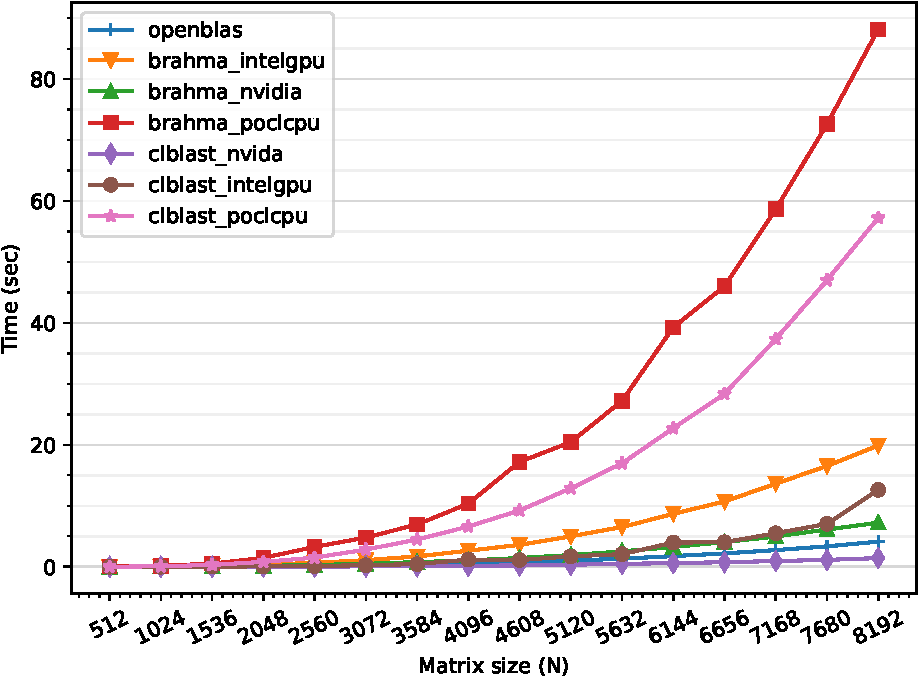
\includegraphics[width=0.45\textwidth]{../data/Lenovo-T480_crop.pdf}
  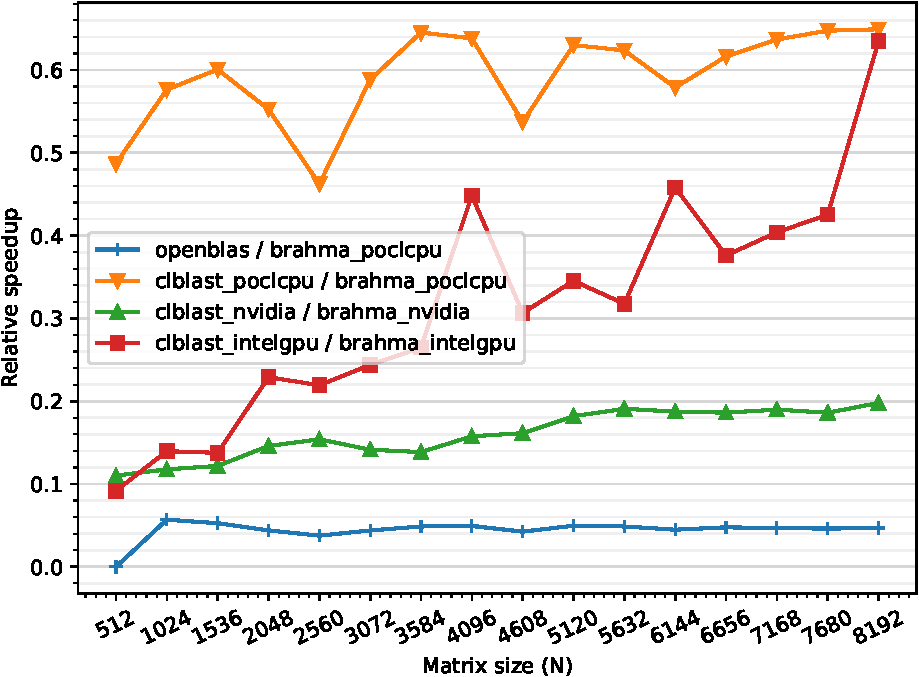
\includegraphics[width=0.45\textwidth]{../data/Lenovo-T480_rel_crop.pdf}\\
  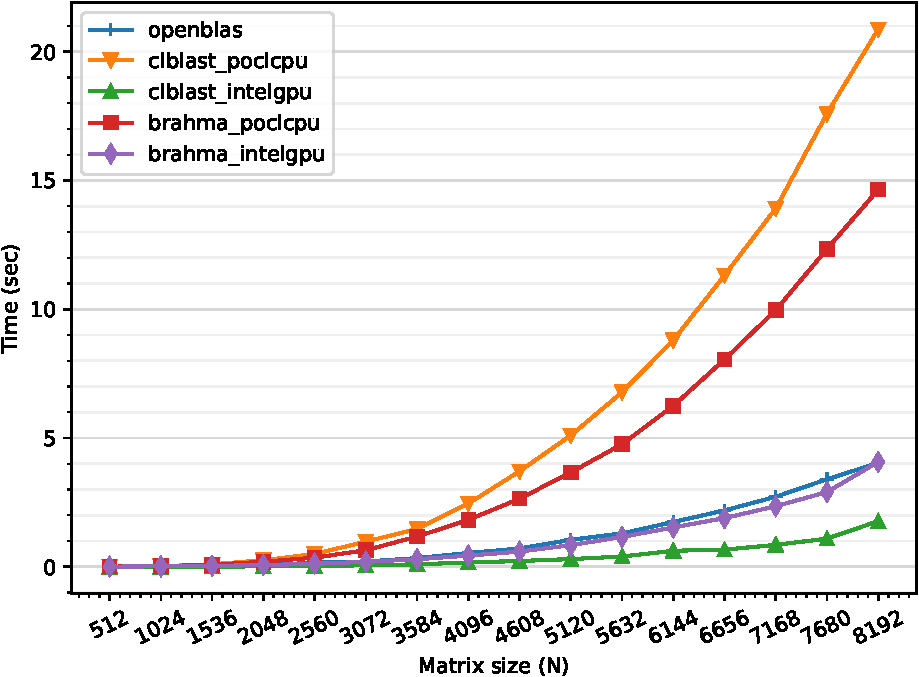
\includegraphics[width=0.45\textwidth]{../data/zenbook_iris_crop.pdf}
  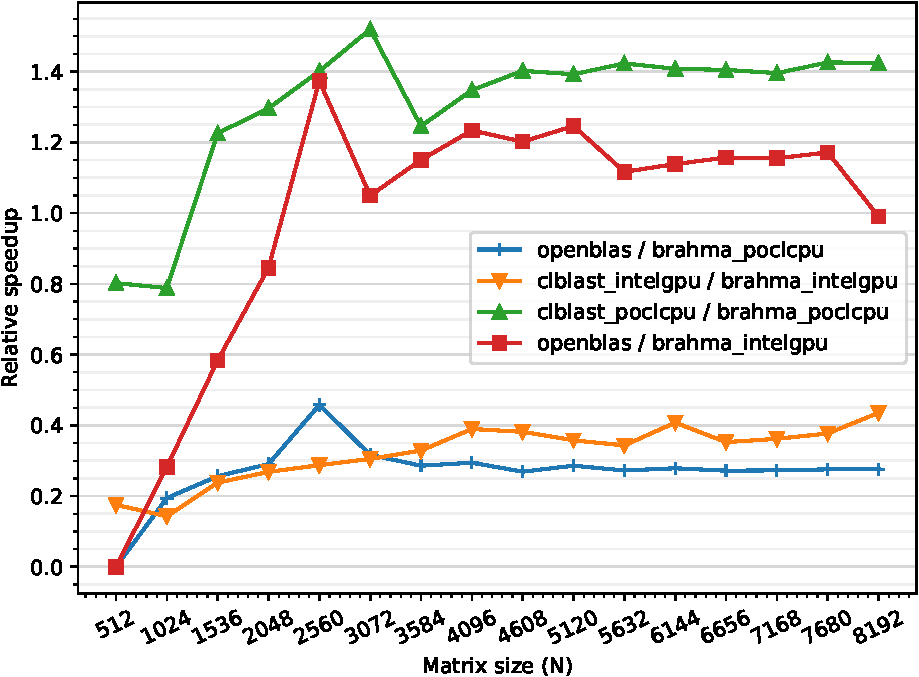
\includegraphics[width=0.45\textwidth]{../data/zenbook_iris_rel_crop.pdf}\\
  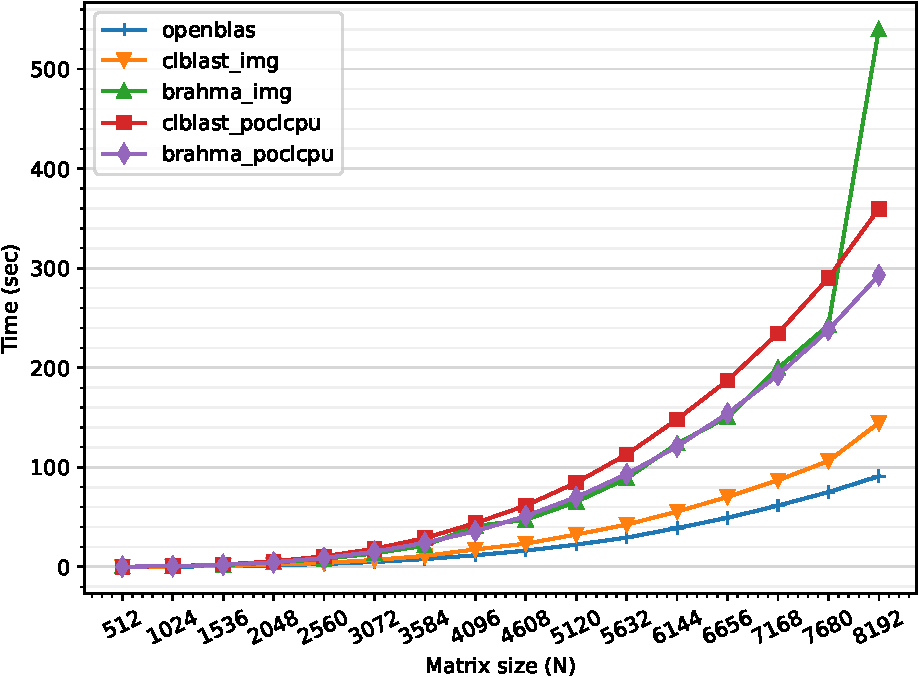
\includegraphics[width=0.45\textwidth]{../data/MILK-V_crop.pdf}
  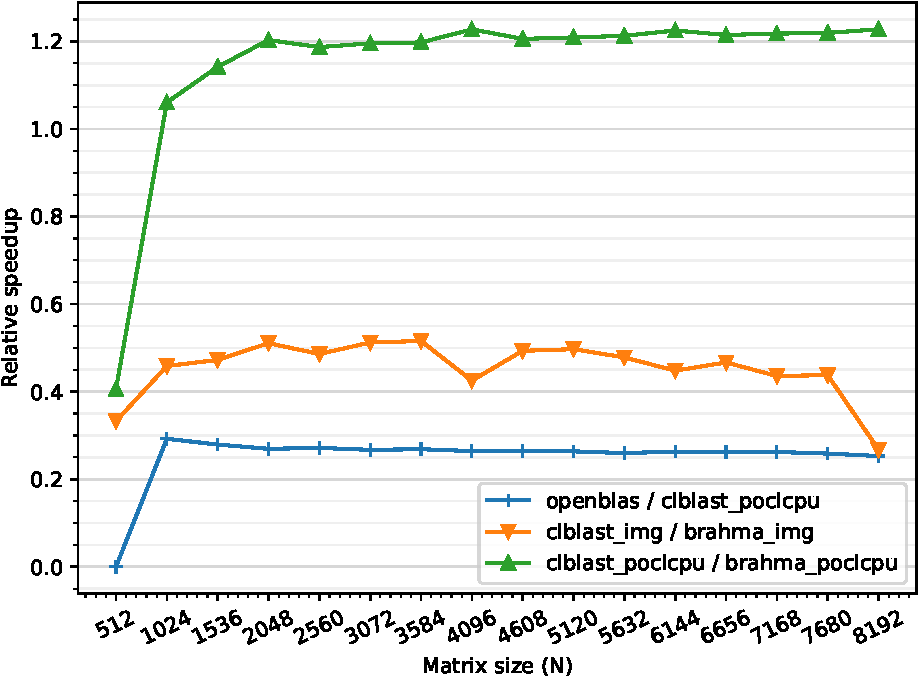
\includegraphics[width=0.45\textwidth]{../data/MILK-V_rel_crop.pdf}
  \end{center}
  \caption{Matrix multiplication performance: 1st row for \textbf{Lenovo}, 2nd for \textbf{Zen}, 3rd for \textbf{MILK-V}}
  \label{fig:mxm_perf}
\end{figure}

We choose two competitors.
The first one is the CLBlast\footnote{CLBlast source code: \url{https://github.com/CNugteren/CLBlast}}~\cite{10.1145/3204919.3204924} that is a highly-tuned (even for low-power mobile GPUPUs) OpenCL-based BLAS implementation.
The second one is the OpenBLAS\footnote{OpenBALAS source code: \url{https://github.com/OpenMathLib/OpenBLAS}} that is a highly-tuned BLAS implementation for CPU.
Additionally, we run OpenCL-based solutions on CPUs using POCL~\cite{Jskelinen2014}.
All competitors were compiled and run with default settings.


We evaluate all competitors on several platforms listed below.
\begin{itemize}
  \item \textbf{Lenovo}: Intel Core i7-8550U CPU, NVIDIA GeForce MX150 and Intel UHD Graphics 620 GPUs.
  \item \textbf{Zen}: Intel Core i5-1340P CPU, Intel Iris Xe Graphics G7 80EUs GPU.
  \item \textbf{MILK-V}. SpacemiT M1 CPU, IMG BXE-2-32 GPU.
  %\item \textbf{OrangePi}, Mali, ARM
\end{itemize}

We generate random square matrices with elements of type \texttt{float32} and use typical arithmetic semiring because our competitors do not provide generic kernels.
Time is measured as an average of 10 runs.
We measure time of client function execution, so it includes data transfer.
Results of evaluation represented in figure~\ref{fig:mxm_perf}: we show both time and relative speedup.

First of all, we show that Brahma.FSharp allows one to create portable solutions.
Obviously, our kernel is not such optimized as kernel from CLBlast, but relative speedup analysis shows that more tuning required: in much cases performance gap decreases with data size increase (\textbf{Lenovo} esp. Intel GPU; \textbf{Zen}).
But in some cases behavior is more complex: for \textbf{MILK-V} our solution on CPU using POCL demonstrates better performance that CLBlast, but on respective GPU performance gap slightly increases with data size increase.

Such behavior can be explained by differences in kernel tuning, but not by the Brahma.FSharp technology problem.
So, while it is unlikely possible to hide dotnet overhead fully, it looks possible to minimize it to be comparable with competitors on big matrices.
To do it we should to create finer tuned and more flexible kernel to allows one better fit performance-affecting parameters.